\documentclass{article}
\usepackage[utf8]{inputenc}
\usepackage{graphicx}
\usepackage{listings}
\title{Information System - Lab work 8}
\author{Tran Thi Hong Hanh}
\date{10 November 2017}

\begin{document}

\maketitle
\section*{Database}

\begin{itemize}
	\item Which normal form does the employee database sastisfy?\\
The database also satisfies Third Normal Form (3NF) since there are no columns that are non-transitively dependent on the primary key and you can infer information from other table using foreign keys.

\end{itemize}

\section*{Normalization}
\begin{itemize}
	\item Produce a 3NF of the following Order form document by normalization.
\begin{figure}[h]
\centering
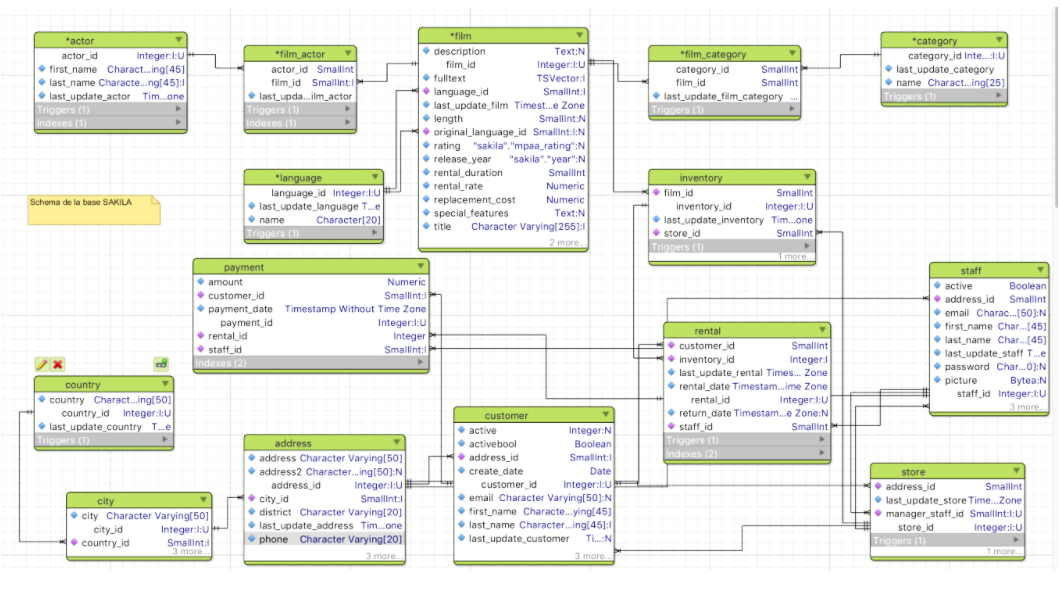
\includegraphics[scale = 0.5]{schema.PNG}
\caption{Databases}
\end{figure}

\end{document}
